\documentclass[a4paper]{article}



%% Language and font encodings
\usepackage[english]{babel}
\usepackage[utf8x]{inputenc}
\usepackage[T1]{fontenc}
\usepackage[compat=1.0.0]{tikz-feynman}

%% Sets page size and margins
\usepackage[a4paper,top=3cm,bottom=2cm,left=3cm,right=3cm,marginparwidth=1.75cm]{geometry}

%% Useful packages
\usepackage{amsfonts}
\usepackage{amsmath}
\usepackage{graphicx}
\graphicspath{ {./img/} }
\usepackage[colorlinks=true, allcolors=blue]{hyperref}
\usepackage{float}
\usepackage{enumerate}
\usepackage{subfig}

\title{REYES Nuclear Physics Mentoring Week 2}
\author{Aman Kumar}

\begin{document}
\maketitle
\section{Introduction}
In week 2 we began our discussion on complex numbers and why it's needed to explain our real world. Although our world is real
we need complex numbers to explain most of the things as the complex nature is most fundamental which makes it easier for us to explain things uding it.
 
One such example of an event in our world which is of our interest is scattering.
\section{Scattering}
Scattering theory is a framework for studying and understanding the scattering of waves and particles.

We need complex numbers to study scattering amplitudes given by $\mathbb{M}$

Here the probability of an interaction to occur is given by $Prob \propto |\mathbb{M}^{2}|$

Also,  $ |\mathbb{M}^{2}| = \mathbb{M}^{\dagger} \mathbb{M} $

and $ \mathbb{M} = \mathbb{M} (\mathbb{E}^{\star})  $ where $\mathbb{E}^{\star}$ is Center of Momentum Energy.

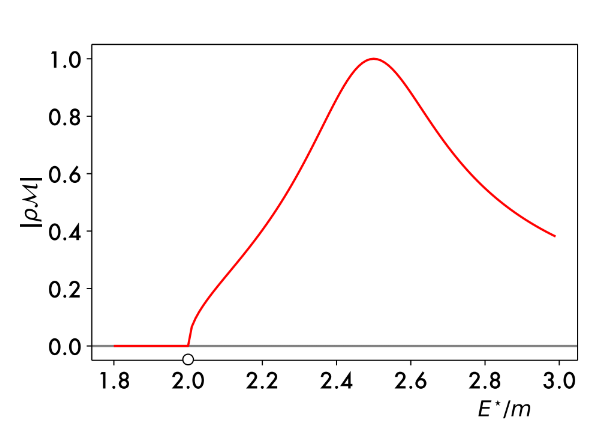
\includegraphics{aimg}


$ \rho $ is known as kinematic factor "phase space".

\section{More}

More work from week two is in the code folder.
\end{document}